This section describe Ascent's primary abstractions and surveys its general capabilities.
%
Ascent organizes its capabilities into five types of in situ tasks, which
it refers to as \textbf{actions}.
%
Its five actions are:
\begin{itemize}
\item \textbf{Pipelines} transform data from one form to another.
%
\item \textbf{Scenes} render images.
%
\item \textbf{Extracts} are used to move data out of Ascent, i.e., to file I/O or to another framework.
%
\item \textbf{Queries} provide quantitative summarizations of the data.
%
\item \textbf{Triggers} adapt when other actions are executed, based on the conditions of the simulation.
%
\end{itemize}

These actions are highly interoperable, and Ascent can employ multiple actions of the same type
at once.
%
Consider the following example of Ascent doing in situ analysis on an input data set, $D$,
for a given cycle of a simulation.
%
Ascent begins by applying an isosurfacing operation to $D$ to make a new data set $D'$ (pipeline).
%
It then applies a trigger to $D'$ --- it takes the surface area of the isosurface (query) and compares
the total area with the area from the previous time it was executed.
%
If the total area has changed by more than 5\%, then Ascent would render an image of $D'$ (scene)
and also save the original data set $D$ to disk (extract).
%
Going beyond this example, it is possible to have multiple triggers, arbitrary conditions for
the triggers (queries or otherwise), as well as many pipelines, scenes, and extracts.
%
Figure~\ref{fig:ascent_example} shows an example of this, specifically two pipelines and two extracts.

\begin{figure}
\centering
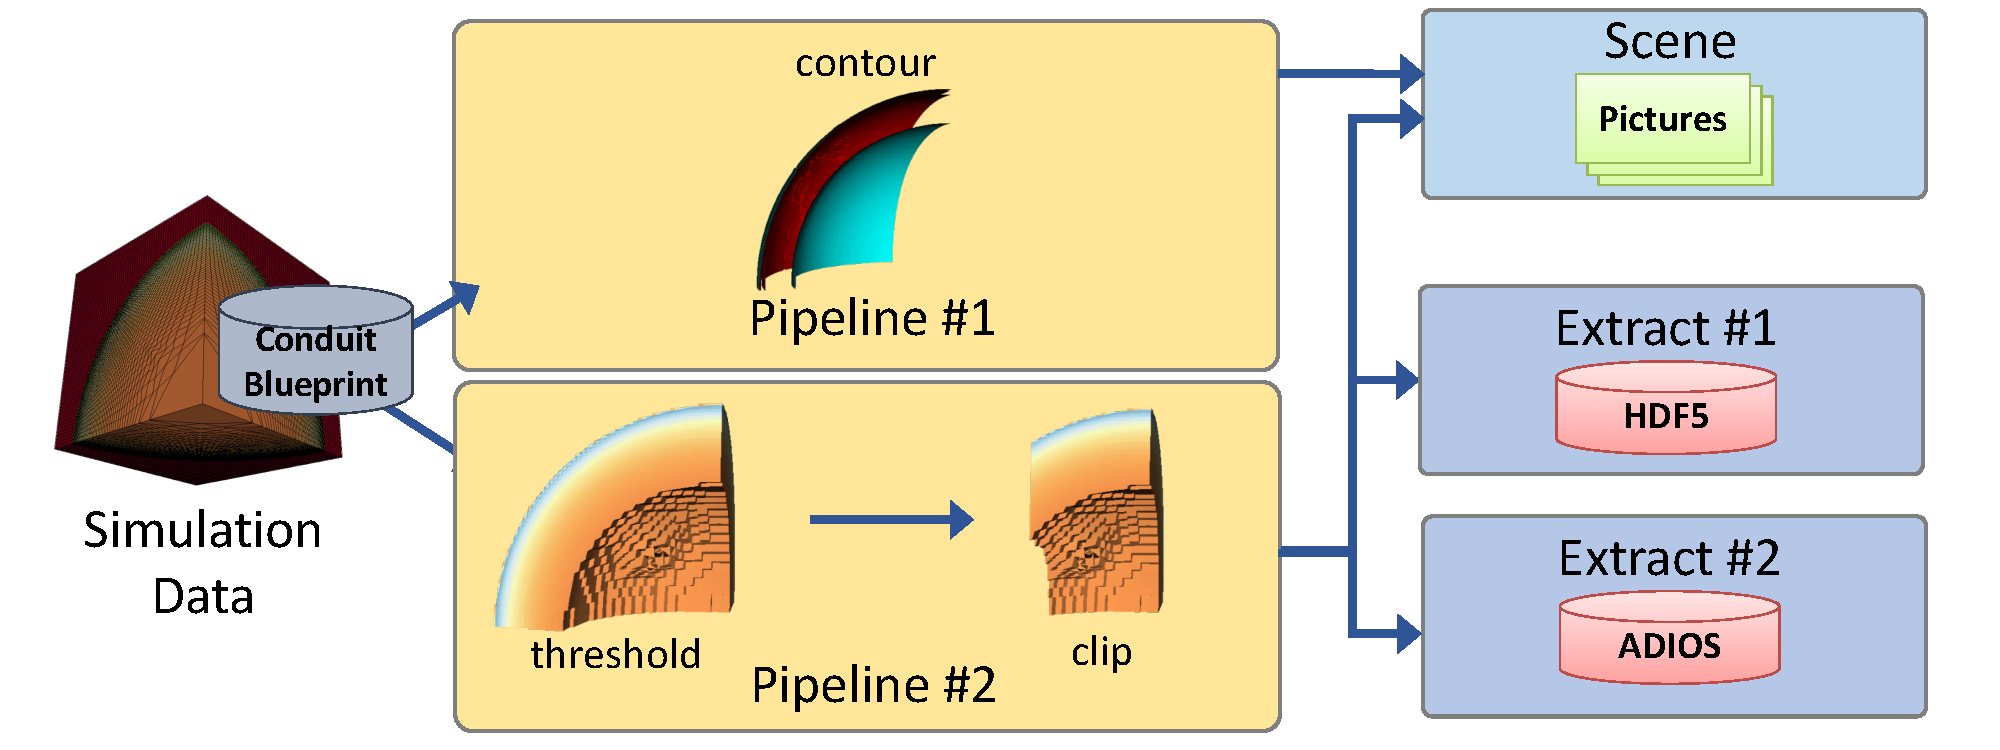
\includegraphics[width=\textwidth]{images/ascent_actions_diagram.pdf}
\caption{\label{fig:ascent_example} An example of how Ascent actions can be combined.
In this example, simulation data is acquired from Conduit/Blueprint (see \S\ref{sec:API}),
and that data is relayed into two pipelines (labeled \#1 and \#2).
The first pipeline applies a contour operation, while the second
applies threshold and clip operations.
%
The results of these pipelines are used in multiple ways.
A scene uses both pipelines as input, while two extracts use only the second pipeline
as input, outputting using two different I/O libraries.}
\end{figure}

\subsection{Pipelines}

Pipelines allows users to describe a series of data transformations, also known as filters,
to execute on simulation data.
%
%These data transformations are sometimes referred to as filters in other
%frameworks (like VTK~\cite{VTK}), and
Figure~\ref{fig:ascent_example} shows
typical filters for visualization: contour, threshold, and clip.
%Figure~\ref{img:pipelines} shows two examples of pipelines.
%%
%Pipeline \#1 creates contours from a simulation field, and pipeline \#2
%thresholds cells that are within a scalar range then applies a clipping operation.
%
Ascent allows users can define an arbitrary number of pipelines.
%
In terms of inputs and outputs, the input to a pipeline is either
the simulation data or another pipeline, and the outputs of a pipeline
can go to scenes, extracts, and queries.
%
Further, triggers can make use of pipelines, and their relationship is discussed further
in \S\ref{sec:ascent:triggers}.

%
%The default source of pipelines, and all other actions, is the data
%published by the simulation, but all actions can consume the results
%of declared pipelines, including other pipelines.

%\begin{figure}
%\centering
%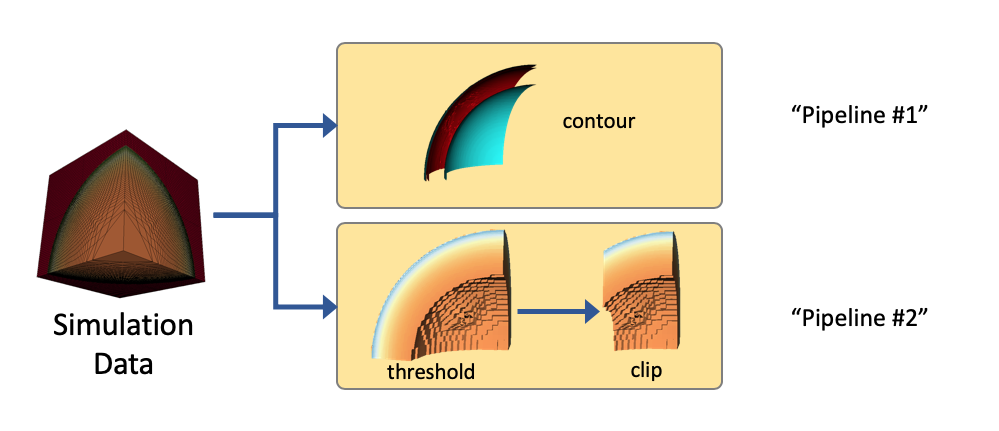
\includegraphics[width=0.6\textwidth]{images/pipelines}
%\caption{\label{img:pipelines} Examples pipelines that transforms simulation data via visualization operators.}
%\end{figure}

Notable filters currently supported by Ascent include:
\begin{multicols}{2}
\begin{itemize}
\item Clipping
\item Contour
\item Histogram
\item Isovolume
\item Particle Advection
\item Statistics
\item Slice
\item Threshold
\end{itemize}
\end{multicols}

There are also filters that create new fields: Divergence, Gradient, Logarithm, Q-Criterion, Vector Magnitude, and Vorticity.
%
Finally, Ascent contains two specific-to-in-situ filters that
reduce data size significantly enough that it can be saved to disk and explored post hoc:
Lagrangian Flow and Sampling (\fix{should be a reference here to Biswas chapter on sampling}).


\subsection{Scenes}

Scenes create images.
%
They typically operate on the output of pipelines, but they also can work directly
on the original simulation data.
%
Scenes do not return anything to Ascent that can interact with other actions, but they
do save the images they produce to disk for later inspection.

A scene is made up of ```renders''' and ```plots.'''
%
Renders can be thought of as sub-scenes, i.e., each scene is made up of many sub-scenes (renders),
which contain
camera specifications, image dimensions, background and
foreground colors, annotation controls.
%
There is no limit to the number of renders for a scene, and there can also be zero.
%
Plots are the things to render.
%
A plot consists of two things: what data to render and how to render it.
%
The data comes from the input pipeline, and the method for rendering it can vary.
%
Currently, Ascent supports four plot types: pseudocoloring, volume rendering, mesh plots,
and radiograph plots(see Figure~\ref{fig:ascent_plots}).
%
Each of these plot types contain parameters that control the input data
(name of the pipeline to consume, which scalar field to operate on, etc.)
and how to carry out the rendering (color tables, scalar ranges, etc.).
%

\begin{figure}
\centering
  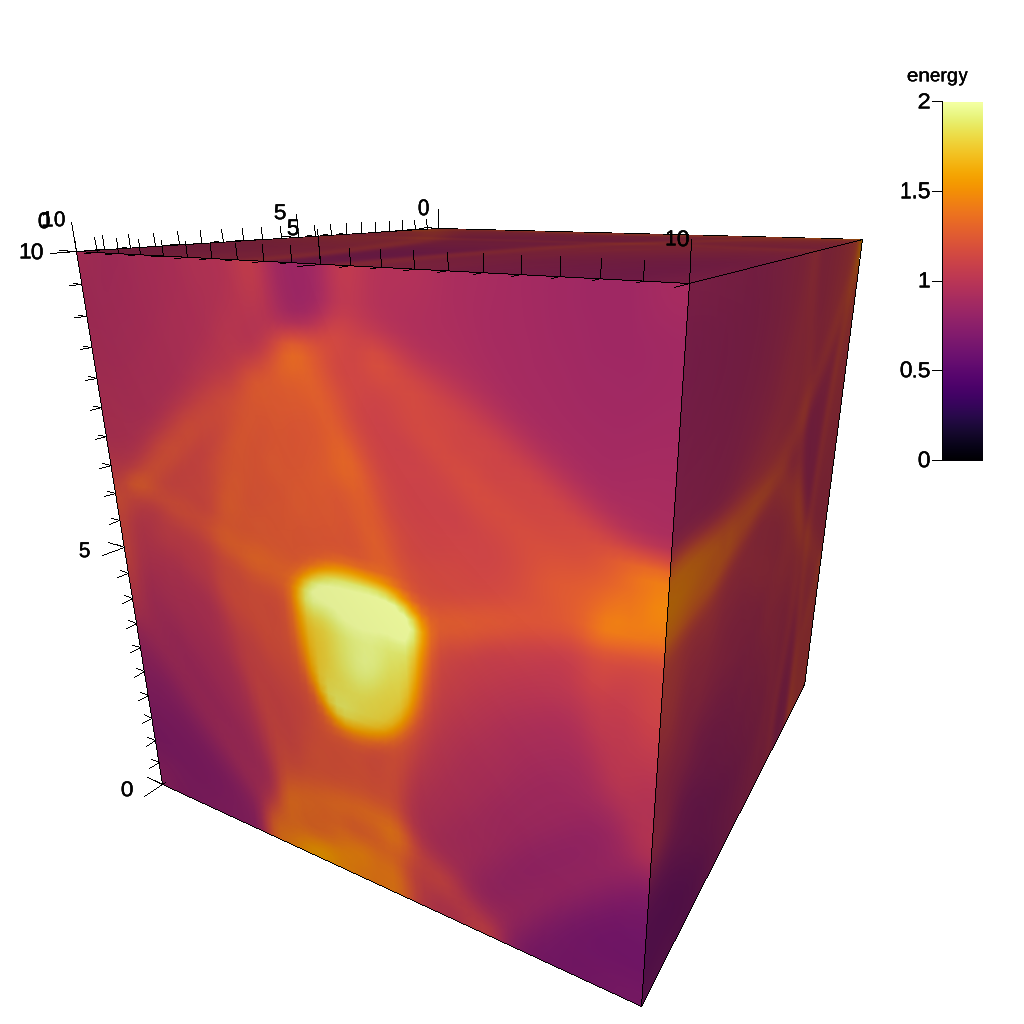
\includegraphics[width=0.4\textwidth]{images/pseudocolor250}
  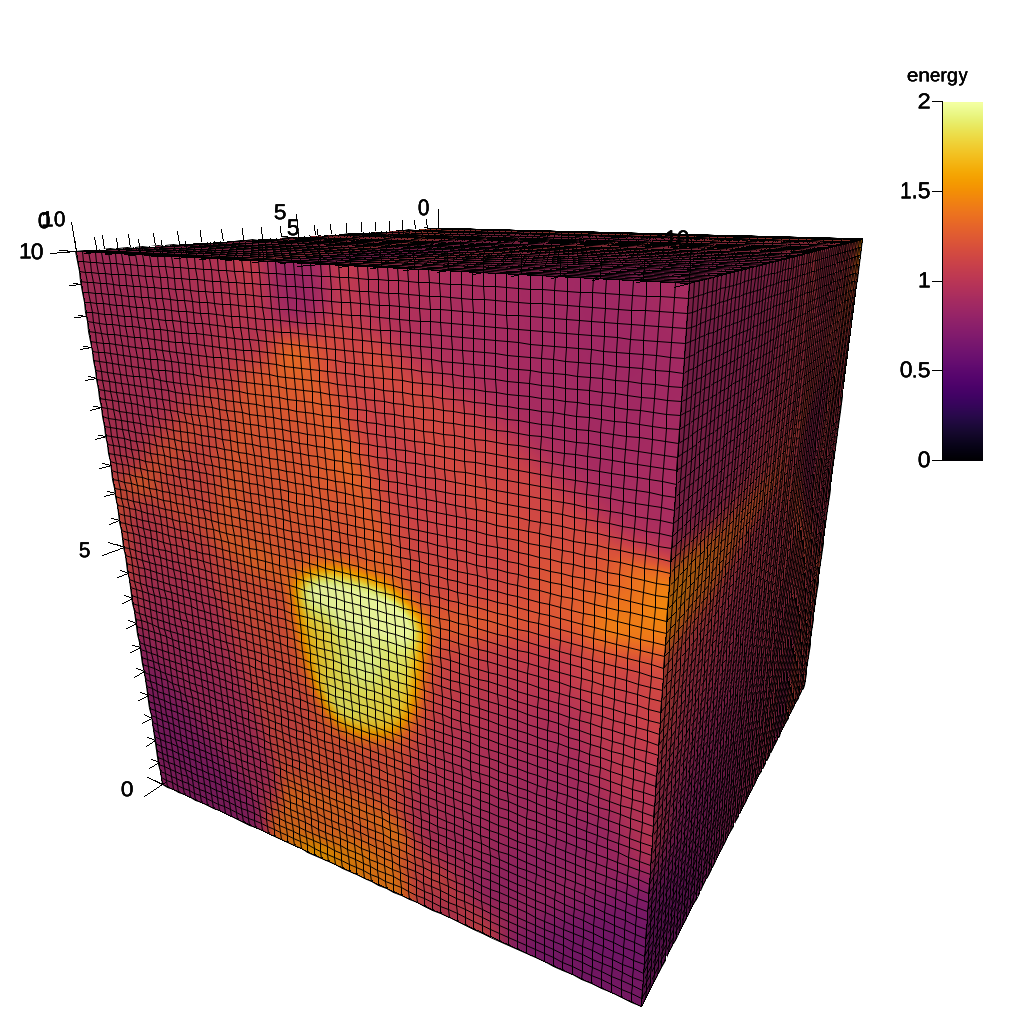
\includegraphics[width=0.4\textwidth]{images/mesh250}
  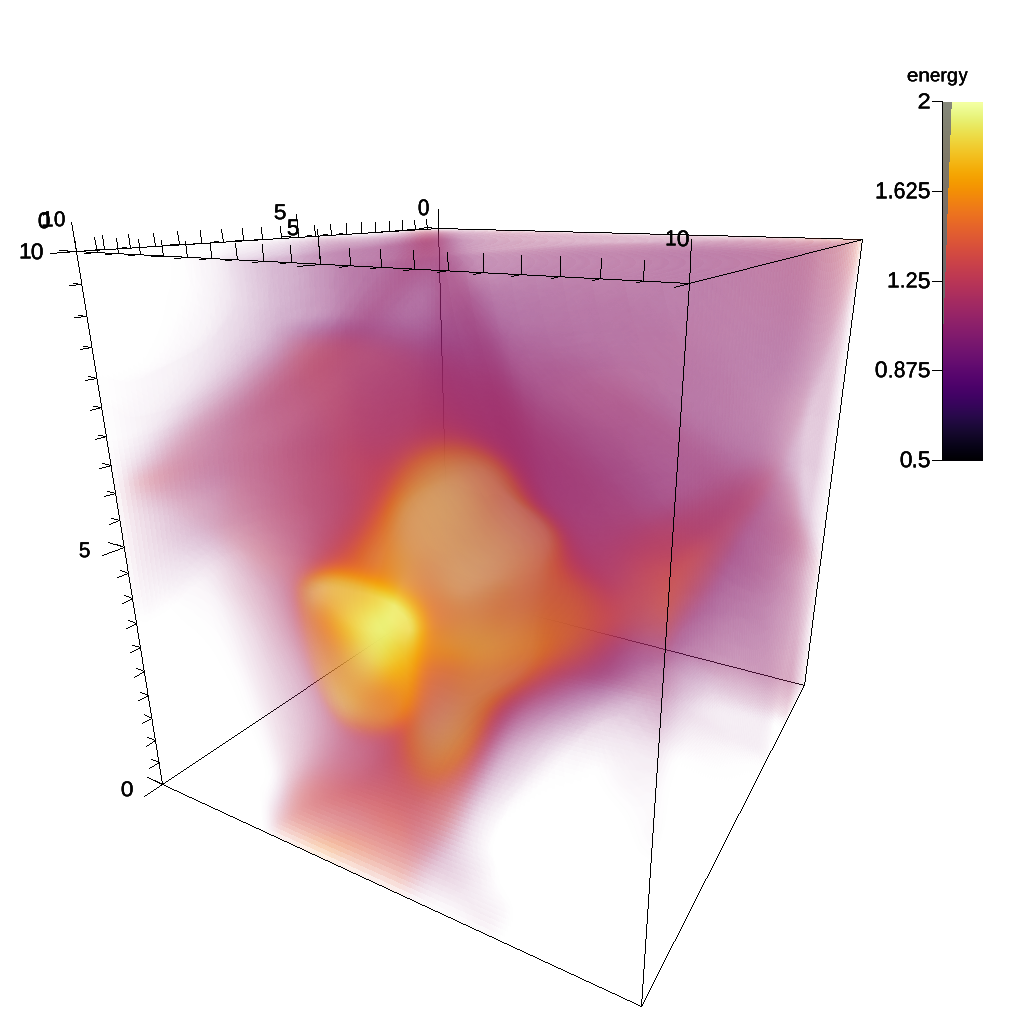
\includegraphics[width=0.4\textwidth]{images/volume250}
  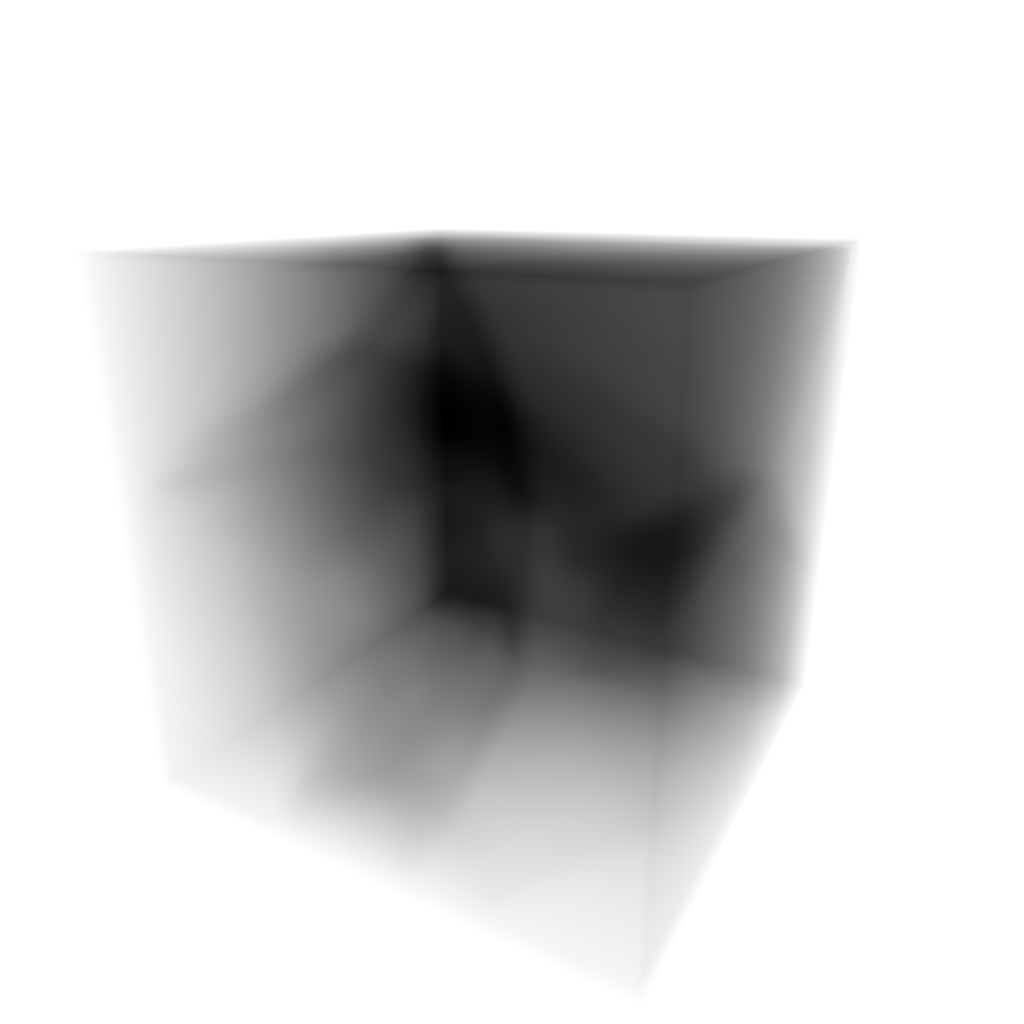
\includegraphics[width=0.4\textwidth]{images/radiograph250}
  \caption{\label{fig:ascent_plots} Example plots used in Ascent scenes.
%
On the top left, a pseudocolor plot, and
on the top right, a pseudocolor plot with a mesh plot.
%
On the bottom left, a volume plot, and
on the bottom right, a radiograph plot.
  }
\end{figure}

In terms of camera placement,
Ascent creates a default camera based on bounding box of the data set and
is always facing the data set.
%
Renders inherit the default camera parameters, which simplifies creating
cameras that actually look at the data set.
%
Ascent also provides simple controls to rotate the camera on the
sphere circumscribing the data set.
%
Of course, the user is free to set all
camera parameters explicitly as well.

Finally, scenes can create Cinema~\cite{AhrensCinema} databases that
create a large set of images that can be explored after the simulation.
\fix{Should be a reference to Cinema chapter here.}

%Currently supported plots include:
%\begin{itemize}
%\item Pseudocolor
%\item Mesh
%\item Volume
%\item Radiograph
%\end{itemize}

\subsection{Extracts}
The extracts action covers a broad range of activities.
%
The common theme between these activities is moving data outside Ascent.
%
The word extract is meant to convey ``extracting'' data from Ascent to somewhere else.
%
%
%Extracts are an escape hatch in Ascent that enables data to be sent
%outside of Ascent.
%
Extracts can be as simple a saving data to HDF5 files.
%
That said, extracts are also the mechanism to integrate other tools with Ascent --- a gateway
to a larger workflow.
%
This is important because
Ascent does not have the long tail of functionality that tools like ParaView or VisIt provide, which
were built over decades of development.
%
Through extracts, Ascent can pass data directly to ParaView Catalyst~\cite{Catalyst}.
%
Another example of using extracts to provide additional functionality is the
ADIOS~\cite{Lofstead2008} extract, which allows Ascent to link to in transit workflows.

Ascent supports connections to the Python ecosystem through the Python and
Jupyter extracts~\cite{CyrusISAV,Jupyter}.
%
Python extracts execute custom analysis code provided by the user, and the
Jupyter extracts allow for incoming Jupyter notebooks connections from a web
browser.

We feel that the Jupyter notebook interface is an important future direction
for Ascent, and for in situ as a whole.
%
One of in situ's greatest weaknesses is the reliance on a priori
knowledge, and one strategy to mitagate this weakness is incorporating a human-in-the-loop.
%
Through the Jupyter notebook interface, users can pause a running simulation
and interact with the data.
%
Additionally, Jupyter widgets enable fast prototyping of domain specific GUIs.

Currently supported extracts include:
\begin{itemize}
\item ADIOS
\item Babel Flow~\cite{babelflow}
\item Jupyter Notebooks
\item ParaView Catalyst
\item Python
\end{itemize}

\subsection{Queries}
\label{action_queries}
Queries enable users to ask quantitative questions.
%
The inputs to a query can take a varied form:
the simulation data directly,
data produced by a pipeline,
or even a combination of multiple pipelines and simulation data.
%
That said, typical queries are used to access the current state of the simulation
and to summarize data.
%
The results of queries are saved in Ascent's state.
%
These results can then be used to
interact with other actions --- a query's return value can be turned
into the parameter for another action (for example setting the camera position in a scene based
on the result of a bounding box query) or it can be used to affect triggers.
%

The mechanism behind queries enables powerful operations.
%
Queries are formed via a Python-like language that
enables expressions for math operations,
call functions, and evaluating conditionals.
%
Further, since the results of queries are stored into named identifiers, subsequent queries
can build on the results of other queries, allowing for complex combinations.
%
%Examples include min-max queries, statistics, cell locations,
%and probability distributions.
%
This also enables creating a ``time history,'' since
Ascent can call the same query every time step and accumulate the result.

%Queries are executed each time Ascent is called, and the resulting time
%history can be saved, accessed by the simulation, or accessed in other
%expressions.

%Queries can be as simple as calling a function that returns the current simulation cycle
%and storing it into a variable.
%
%More complex queries can calculate the amount of entropy of a field.
%

Examples of queries include:
\begin{itemize}
\item $cycle()$: calling a function that return the current simulation cycle and storing it into a variable.
\item $max(field('pressure'))$: the maximum value of the pressure field.
\item $entropy(histogram(field('gyre'), num\_bins=128))$: calculating a histogram of the gyre field with 128 bins, and then calculating the entropy of that histogram.
\end{itemize}
%Listing~\ref{simple_query} shows the declaration of a query that returns
%the current simulation cycle and stores it into a variable identifier \textit{cycle},
%and Listing~\ref{complex_query} shows a more complex example of a query that
%calculates the entropy of a simulation field.
%\begin{lstlisting}[language=Python,caption={Examples of querying the simulation cycle}, label={simple_query}]
%# add a simple query expression (q1)
%queries["q1/params/expression"] = "cycle()"
%queries["q1/params/name"] = "cycle"
%\end{lstlisting}
%

%
%
%\begin{lstlisting}[language=Python,caption={A more complex example of queries in Ascent}, label={complex_query}]
%# add a more complex query expression (q2)
%queries["q2/params/expression"] = "entropy(histogram(field('gyre'), num_bins=128))"
%queries["q2/params/name"] = "entropy_of_gyre"
%\end{lstlisting}

\subsection{Triggers}
\label{sec:ascent:triggers}

In a typical scenario, in situ visualization is performed at regular intervals, e.g.,
every $X$ simulation cycles or every $M$ minutes of wall clock time.
%
This approach creates a tension between two important goals:
(1) achieving the visualizations and analyses at the right times within the simulation
and (2) minimizing costs.
%
On the one hand, performing visualization frequently maximizes the chances of having
visualizations at the right times (and likely also some uninteresting times), but
is costly,  e.g., adding a 50\% overhead on top of the simulation.
%
On the other hand, performing visualization infrequently minimizes costs, but also makes it
less likely that the visualizations will occur during important phenomena.
%

``Triggers'' are designed to balance the tensions between cost and capturing important phenomena.
%
Triggers operate in two phases: inspection and action/inaction.
%
The purpose of the inspection phase is to determine if the action should be taken, if so, then
the trigger should ``fire.''
%
Further, if the inspection routine is cheap (i.e., executes quickly) and accurate (i.e.,
fires at the right times), then
triggers can be an effective strategy.
%
In this case, triggers can be called frequently (possibly every cycle) and still minimize cost
(since the visualization in the action/inaction phase is called only when necessary) and
get the right information (since the trigger is accurate).
%
Of course, triggers make the most sense when the desired visualization is quite expensive
to calculate;
if the desired visualization could be calculated as quickly as the trigger, then there would
not be a cost benefit.





%Traditional in situ actions execute every $X$ simulation cycles, this presents
%two related problems.
%
%First, if the analysis is expensive, then the total cost of the action may exceed
%what a user is willing to pay,
%
%Second, if the analysis called infrequently, then the feature or event that the analysis is
%trying to capture could easily be missed.
%
Triggers address these issues by coupling inspection routines with analysis, and a
potentially costly analysis only executes when user defined precondition is met.
%
Ideally, inspection routines are cheap and can be called every cycle, while the analysis
that are ``triggered'' can cost more.

Ascent triggers builds on the queries and expression support introduced in
Section~\ref{action_queries}, and the trigger condition can be any conditional
expression.
%
When the condition evaluates to true, the trigger fires, executing a user provided
set of actions, which can be any Ascent action.
%
Triggers can be used to execute actions for debugging purposes(i.e., saving data to
a file when invalid values are found) or rendering images when a large
change is found(i.e., when the max value of a field exceeds a threshold from the
previous value).
%
When an event can be expressed in these terms, triggers are a powerful tool for
maximizing constrained resources in situ.

Example of triggers include:
\begin{itemize}
\item $cycle() > 100 \ and \ cycle() < 200$
\item $max(field('pressure')) > 100.0$
\item $magnitude(max(field('braid')).position - vector(0,0,0)) > 0$
\end{itemize}
